%description: Math 290 HW Template

%%%%% Beginning of preamble %%%%%

\documentclass[12pt]{article}  %What kind of document (article) and what size

%Packages to load which give you useful commands
\usepackage{subfig}
\usepackage{graphicx}
\usepackage{hyperref}
\usepackage{amssymb, amsmath, amsthm}

%Sets the margins

\textwidth = 6.5 in
\textheight = 9 in
\oddsidemargin = 0.0 in
\evensidemargin = 0.0 in
\topmargin = 0.0 in
\headheight = 0.0 in
\headsep = 0.0 in
\parskip = 0.2in
\parindent = 0.0in

%defines a few theorem-type environments
% \newtheorem{theorem}{Theorem}
% \newtheorem{corollary}[theorem]{Corollary}
% \newtheorem{definition}{Definition}

\newtheorem{definition}{Definition}
\newtheorem{fact}{Fact}
\newtheorem{remark}{Remark}
\newtheorem{theorem}{Theorem}
\newtheorem{proposition}{Proposition}
\newtheorem{lemma}{Lemma}
\newtheorem{corollary}{Corollary}

\renewcommand{\labelenumi}{\arabic{enumi}.}
\renewcommand{\labelenumii}{\arabic{enumi}.\arabic{enumii}.}
\renewcommand{\labelenumiii}{\arabic{enumi}.\arabic{enumii}.\arabic{enumiii}.}
\renewcommand{\labelenumiv}{\arabic{enumi}.\arabic{enumii}.\arabic{enumiii}.\arabic{enumiv}.}
\newlength{\alginputwidth}
\newlength{\algboxwidth}
\newcommand{\alginput}[1]{\makebox[1.5cm][l]{ {\sc Input:}} \parbox[t]{\alginputwidth}{{\it #1}}}
\newcommand{\algoutput}[1]{\makebox[1.5cm][l]{ {\sc Output:}} \parbox[t]{\alginputwidth}{{\it #1}}}
\newcommand{\algtitle}[1]{\underline{Algorithm \ {\bf #1}} \vspace*{1mm}\\}

%%%%% End of preamble %%%%%







\begin{document}

\title{AI for Risk Game}

\author{
{Wah Loon Keng}\thanks{
Lafayette College,
Easton, PA 18042, USA.
kengw{\tt @}lafayette.edu.}
\qquad
{Benjamin H. Draves}\thanks{
Lafayette College,
Easton, PA 18042, USA.
dravesb{\tt @}lafayette.edu.}
      % \affaddr{Department of Computer Science}\\
%       \affaddr{Lafayette College}\\
%       \affaddr{Easton, PA 18042, USA}\\
%       \email{gexia@cs.lafayette.edu}
}
% \date{}
\maketitle

\begin{abstract}
We implement an AI to play the board game $\emph{Risk}$. The game is formalized as an optimization problem in graph theory, where countries are represented as nodes in an undirected graph, and decisions are considered based on the graph properties. We introduce solution algorithms, with variable parametrizations, which are then implement as AIs with different personalities in {\tt JavaScript}. We set up games among AIs to measure their performances, and discover unusual game strategies.
\end{abstract}










\section{Introduction} \label{intro}

The board game $\emph{World Domination RISK \circledR}$ is a game of military strategy, where players of different factions try to conquer all 42 countries on the map, by deploying armies to attack and defend. We use the classic $\emph{Hasbro}$ version of the game; the rules are well known and can easily be found online, but they will be included as we walk through our algorithms.

In this paper, we first set up our formalization of the game as a graph optimization problem. Next we introduce graph algorithms to carry out each of the game moves, and explain our reasoning behind them. Then, we combine these to implement an AI, with variable personalities based on the parametrization of its internal algorithms. The different AIs then play multiple games against one another, with their results recorded. Finally, we analyze their performances, and find several unusual, interesting strategies discovered by the AIs that are never observed from human players.

This entire project is public on GitHub: \url{https://github.com/kengz/Risk-game}.



\section{Formalization} \label{formalization}

The game is inherently dependent on the board, which is a world map of 42 countries, interconnected in specific ways. Decisions to attack or defend are based on the distribution of the armies, the surroundings of a location, and connectivity of countries. These motivate our formalizing the game board and algorithms based on an undirected graph. From now we shall refer to the graph representation as $\emph{map}$:

\begin{definition} \label{map}
A $\textbf{map}$ is a connected, undirected planar graph, with 42 nodes, each representing a country. The nodes are named with indices $0-41$, and are connected the same way as are countries on the game board by undirected edge of weight 1.
\end{definition}

We assign data fields to each node, namely its country name, the continent it is in, its player owner, the number of armies of the owner in it, its worth and pressure as determined by some metric described below.


\begin{definition} \label{region}
A $\textbf{region}$ is a connected subgraph consisting of nodes all owned by the same player. Each player can own many regions, which together partition the map.
\end{definition}

\begin{definition} \label{border}
A $\textbf{border}$ node of an AI is its node that is adjacent to at least an enemy node.
\end{definition}

\begin{definition} \label{attackable}
A $\textbf{attackable}$ node for an AI an enemy node adjacent to its border.
\end{definition}

\begin{definition} \label{shape}
The $\textbf{shape}$ of a region is the measure of its shape/roundess. To compute the shape, find the maximum and minimum distances between the border nodes in the region, and shape=(max-min)/max. If a region is round, shape = 0; if it is a line, shape = 1.
\end{definition}

\begin{definition} \label{radius}
$\textbf{Radius}$ is the measure of shortest distance from an origin node. We identify the neighbors of node $\mathcal{O}$ at radius k to be the nodes whose shortest distance from $\mathcal{O}$ is k.
\end{definition}


Furthermore, we define the fields that will be useful in our algorithms:

\begin{definition} \label{worth}
The $\textbf{worth}$ of a node is the measure of its importance to an AI, as calculated by its internal metric algorithm, and is used by the AI to prioritize its decisions: which node should it defend/attack first.
\end{definition}

\begin{definition} \label{pressure}
The $\textbf{pressure}$ of a node as perceived by an AI is the measure of the average army distribution around the node, up to 5 unit radii away. It is calculated by the AI's internal metric and used to prioritize decisions.
\end{definition}

Note that the worth and pressure of a node are not the same when calculated by opposing AIs due to different perceptions, metric and AI personalities. Each AI will be calculating these values for all 42 nodes at each turn.

Finally, we introduce a data structure as the raw representation of overall army distribution on the map for various calculations:

\begin{definition} \label{RMAM}
The $\textbf{Radius Matrix (RM)}$ from an origin node $\mathcal{O}$ is the matrix that better represents the connectivity of neighbor nodes of the origin within some radius. It is enumerated by the Radius Matrix Algorithm below, and each entry is the name of some node.

Its corresponding $\textbf{Army Matrix (AM)}$ is a different representation of the RM, with each entry now being $z \in \mathbb{Z}$, where $|z|$ is the number of armies at the node, and $z$ is positive if the node is owned by the calculating AI, and negative otherwise.
\end{definition}







\section{Algorithms}

We now enumerate the algorithms for each step of the game, which will collectively form the final algorithm used by the AI to play the game.


\subsection{The Matrix Algorithms}

\algtitle{Radius Matrix (RM) for an origin node $\mathcal{O}$}
Starting from an origin node $\mathcal{O}$, initialize an empty matrix for its RM,
\begin{enumerate}
	\item Add the index of each adjacent node (at radius 1) of $\mathcal{O}$ to a new row in RM.
	\item Repeat for $i \in \{2,3,...,n\}$, where $n$ is the maximum radius covered:
	
	For each entry $p$ at column $i$, get all $n_p$ of its adjacent nodes at radius $i+1$ from $\mathcal{O}$. 

	\item Duplicate the row of entry $p$ while appending to it each of the $n_p$ adjacent nodes at column $i+1$. If $n_p=0$, append $``empty"$ instead. The process is akin to a Cartesian product.

	\item Return the RM for $\mathcal{O}$.
\end{enumerate}

Note that the column number will coincide with the radius from $\mathcal{O}$. The RM with $n$ columns is a representation of the connectivity from the origin up to radius $n$, where each row is the shortest path from the origin to a point at radius $n$, and there may exist many such paths.

\algtitle{Army Matrix (AM) for an origin node $\mathcal{O}$}
We can convert an RM into AM, a representation using the number of armies,
\begin{enumerate}
	\item Find the RM for node $\mathcal{O}$ using the RM algorithm.
	\item For each entry $p$ in RM, if node $p$ has the same owner as $\mathcal{O}$, replace the entry with the number of army at $p$; else, replace with the negative of the number of army at $p$. If an entry $p$ is $``empty"$, append 0 instead.
	\item return the AM for $\mathcal{O}$.
\end{enumerate}


This transforms an RM into its alternate form AM, which gives a representation of the army distribution and connectivity around the origin node $\mathcal{O}$. This matrix can be used for calculating the $\textbf{pressure}$ from definition \ref{pressure}. For our project we calculate the matrices up to radius 5, which we think is sufficient given that per game turn a player can only move adjacently among nodes.





\subsection{The Pressure Algorithm}

The pressure of each node from an AI's point of view is the average number of army surrounding the node. More positive pressure indicates the node is a better stronghold of the AI; more negative pressure indicates is surrounded by more enemies.

The calculation of pressure depends on the AI's perception of threat, which can be represented using a metric that varies based on its personality.

\begin{definition}
The $\textbf{threat perception}$ of an AI is the way it sees the threat of army distribution up to some radius away poses on an origin node. E.g. 10 enemy armies further away poses less threat than 5 enemy armies nearby. The $\textbf{threat perception}$ is quantified by defining a metric: a normalized vector or length = max radius of AM, where the individual value of the vector is the weight multiplied to the army number at that radius. The procedure is describe below.
\end{definition}

\algtitle{The Metric Algorithm}
To enumerate the metric for an AI's threat perception, with scope radius = 5,
\begin{enumerate}
	\item Choose a weight function, for example, constant, Gaussian,
	\item Evaluate function values for with the input distance vector $\{1,2,3,4,5\}$
	\item Renormalize the output vector and return it as the metric vector.
\end{enumerate}

This metric vector $\mathbf{w}$ is then dotted with a row $\mathbf{r}$ in the AM, which is a list of number of armies at incremental distance away from an origin node $\mathcal{O}$, and the partial pressure $\emph{PP}$ for it is:
$$\emph{PP}(\mathbf{r}) = \mathbf{w} \cdot \mathbf{r}$$


\algtitle{The Pressure Algorithm}
The AI calculates the pressure for each node using its personality trait $\textbf{threat-perception}$, or the metric vector $\mathbf{w}$:
\begin{enumerate}
	\item Update the data fields of the map and call the AM algorithm to compute the AMs for all 42 nodes.
	\item For each node $\mathcal{O}$, compute the dot product between $\mathbf{w}$ and each row of the node's AM; the result is a column vector $\mathbf{c}$.
	\item The first column of the original RM is a repeated list of $m$ adjacent nodes of $\mathcal{O}$, suppose each node $i$ repeats $q_i$ times in the column, so in total the column has length $q_1 + q_2 + \cdots + q_m$. Renormalize this sequence into $nq_1 + nq_2 + \cdots + nq_m$ For each batch $q_i$ of the column vector $\mathbf{c}$ from above, take its mean, then multiply by the renormalized weight $nq_i$. Then sum all $m$ of the results, call this scalar $s(\mathcal{O})$.
	\item Now that the column $\mathbf{c}$ has been reduced to a scalar representing the average army distribution around the origin $\mathcal{O}$, account for the number of armies (sign-sensitive, negative for enemy) here $a(\mathcal{O})$ by adding the scalar, and return the pressure of node $\mathcal{O}$, $P(\mathcal{O}) = s(\mathcal{O}) + a(\mathcal{O})$.
\end{enumerate}


Thus at each turn, the AI updates the data fields and calculates the pressure, i.e. the average number of surrounding armies, for each node, using its threat perception metric.




\subsection{The Worth Algorithm}

\algtitle{The Worth Algorithm}
At each turn, the AI evaluates the worth of each node to prioritize its attacks and defenses. Suppose it considers $m$ factors, each of which assumes a real positive value, with more positive being more worthy. To compute the final worth scalar, simply order the $m$ factors from the most vital, and dot it with a factor vector $\{10^{m-1}, ..., 100, 10, 1\}$.

For our AI, we consider the following factors (ordered from the most important). For each node $\mathcal{O}$ calculate and append to the list of factors:

\begin{enumerate}
	\item continent-fraction = $\frac{\text{(number of nodes with the same owner in the same continent $\mathcal{O}$)}}{\text{(total number of nodes in the continent)}}$
	\item If $\mathcal{O}$ is own node, the region-index: Enumerate for each player its nodes, and group them by regions, then order them from the biggest to the smallest regions. The region-index of $\mathcal{O}$ is its index in this list. Or if $\mathcal{O}$ is enemy, the attackable index: of the region list enumerated above, extract the sublist with nodes that are attackable, i.e. is an enemy adjacent to one of your nodes. The attackable index of $\mathcal{O}$ is its index in this sublist; -1 otherwise.
	\item shape: find the region $\mathcal{O}$ is in and compute the shape as in definition \ref{shape}.
	\item degree: the degree of $\mathcal{O}$, i.e. the number of adjacent nodes it has.
	\item pressure: as calculated from the pressure algorithm.
	\item Finally, return the dot product between this factor list and $\{10^{4}, 1000, 100, 10, 1\}$.
\end{enumerate}


After obtaining an ordered list of worth nodes, we can partition it while preserving the order into lists of border nodes and attackable nodes, and reorder them based on strategies. Furthermore, the AI makes it context-sensitive by remembering the pressures from the past turn, and reorder the list based on pressure-drop between turns.



To justify our factors above, conquering a whole continent gives a player extra armies per turn while strengthening the region. Furthermore, a larger region is harder to attack than a smaller region, thus we place more importance on the nodes there. 

The shape of a region is vital for defense and army mobility during fortification. This is the classic problem of minimizing the surface/volume ratio, or in this lower dimensional case, the perimeter/surface ratio. Intuitively, a thin region is vulnerable, and has bad army mobility. A thick, concentric shape is stronger. The average distance between nodes is also shorter and thus aids mobility. Moreover, a node with higher degree improves mobility since it can reach many other nodes.

The pressure measures the ease of attacking or defending a node; the less negative a node is, the less enemy presence it has. It is wise to not attack the enemy's stronghold, but to seek its weak point of entry, which can be detected from a less-negative pressure.


\subsection{The Priority Algorithm}
At each game turn, the AI updates the priority nodes to attack/defend. The list of priority nodes depends on the AI's personality trait $\textbf{priority}$, whether it is agressive (attack-then-defend) or defensive (defend-then-attack).

\algtitle{The Priority Algorithm}
\begin{enumerate}
	\item Update the data fields for the AI.
	\item Call the pressure algorithm on the map.
	\item Call the worth algorithm on the map.
	\item Repartition the worth nodes and reorder by attackables/borders first based on the AI's personality, whether agressive or defensive. Furthermore, for the attackable, choose the best origin of attack by the highest pressure.
\end{enumerate}







\subsection{The Placement Algorithm}
This describes how the AI places the armies into the its priority nodes based on its personality trait $\textbf{placement}$.

\algtitle{The Placement Algorithm}
\begin{enumerate}
	\item If the trait is $\textbf{cautious}$, place armies along its  priority nodes (if is enemy, use the best origin of attack) until all pressures are $>0$, then with the extra armies, place 4 each down the same list; repeat until none left.
	\item If the trait is $\textbf{tactical}$, place armies down the list until node pressure is $>4$, then with extra, place 4 each down the list; repeat until none left.
\end{enumerate}







\subsection{The Attack Algorithm}
The AI decides to launch attacks from the best attack origin (calculate with in priority list) based on its personality trait $\textbf{attack}$.

\algtitle{The Attack Algorithm}
For all attackables down the priority list,
\begin{enumerate}
	\item If the trait is $\textbf{rusher}$, the AI harassess constantly, i.e. while the best attack origin has 2 more armies than the enemy target, keep attacking before moving to next target.
	\item If the trait is $\textbf{carry}$, same as above, but the difference threshold is 4 (higher). Furthermore, the AI will accumulate the cards to reserve more armies for late game.
\end{enumerate}








\subsection{The Fortifying Algorithm}
All AIs use the same fortifying algorithm.

\algtitle{The Fortifying Algorithm}

\begin{enumerate}
	\item Find the border node $\mathcal{O}$ with the lowest pressure, and find a non-border ally node with higher pressure, transfer all but 1 troop to the border node if possible. This is to always push the unused central forces out to the borders where armies are mostly needed.
	\item If no fortification done above, find a border node with the highest pressure, and transfer any neighboring armies (all but 1) to it. This is for the accumulation of armies during late game by making strong node even stronger.
\end{enumerate}


This algorithm aims to create a center-weak border-strong army distribution within a region with, that is to utilize the maximum number of armies by putting them to the border nodes. Such distribution is efficient for both offense and defense. The second part of the algorithm kicks in when there is less border nodes during the late game, when one player controls a larger region. This will accumulate all armies toward a border node to overwhelm the enemy, hopefully ending the game quicker.







\section{AI Algorithms and Personalities}

We now put everything together to form the AI, which has four personality traits parametrized in its algorithms: 

\begin{enumerate}
	\item The $\textbf{threat perception}$ trait /metric in the Pressure Algorithm; function variations: \{Constant, Survival\}.
	\item The $\textbf{priority}$ trait in the Priority Algorithm; variations: \{agressive, defensive\}.
	\item The $\textbf{placement}$ trait in the Placement Algorithm; variations: \{cautious, tactical\}.
	\item The $\textbf{attack}$ trait in the Attack Algorithm; variations: \{rusher, carry\}.
\end{enumerate}

Thus there are $2^4 = 16$ AI personalities, and more if we allow richer variations.


Corresponding to the game moves per turn:
\begin{enumerate}
\item Getting and placing new armies;
\item Attacking, if you choose to, by rolling the dice; 
\item Fortifying your position (moving troops between an adjacent pair of your nodes),
\end{enumerate}

the AI has these primary methods:
\begin{enumerate}
\item Update: Call the Priority and Worth algorithms.
\item Get-and-Place-Armies: Call the Placement Algorithm.
\item Attack: Call the Attack Algorithm as many times as wanted.
\item Fortify: Call the Fortify Algorithm.
\end{enumerate}



A game can have as many participating AIs as permitted by the rules. During the initial game setup, countries are randomly assigned to the AIs. Then, the AIs take turn to call their Update and Get-and-Place-Armies methods to complete the setup. Then the game begins and the AIs take turn to call all their primary methods in sequence, until the game terminates, or ties at the maximum number of rounds.

As opposed to physical game, the virtual game has no limit on the number of army pieces $-$ it just keeps creating more as needed; nor it has the limit on the cards $-$ it keeps reshuffling a new deck once an old one runs out.


Next we present the results from our implementation.

\section{Implementation Results}

\subsection{Formalization of Problem}
Our initial approach to the problem is one that focuses on the gross number of countries and armies an AI possesses throughout the game. As the game progresses, we monitor how the AI’s interact in their attempt to win both armies and territories based on their personalities. From this, conclusions were drawn regarding personality types, player order effect, as well as game starting conditions. 


\subsection{Algorithms and Decisions}

\subsubsection{Initial Concerns}
An initial issue was normalization of the time axis across several games. While games were initially capped at 100 rounds, where the game was declared a draw, the games that did not end in a draw had variable game length. The majority of the data analysis done in this project was done where there was a definitive winner. From this, the time axis was normalized by considering games in terms of percentage of game length. To the AI the length of the game is unknown during gameplay. However, the analysis can show where pivotal points occur across the game. While initially, players will be unable to use this information an understanding of both territorial and army control will influence their decisions.


\subsubsection{The Difference Plots}
In this analysis, the percentage of both armies and countries in total will be compared to the percentage of the game in where these points occur. These points for players \emph{p1, p2} will be found using the following 
$$\emph{diff\_army} = \frac{\emph{p1\_army - p2\_army}}{\emph{p1\_army - p2\_army}}$$
$$\emph{diff\_country} = \frac{\emph{p1\_country - p2\_country}}{\emph{p1\_country - p2\_country}}$$

This data is stored in a matrix that holds both army numbers and round numbers. In this matrix, data from games resulting in draws is discounted. The equation will hold for any winner. From this we expect a divergent trend from zero as the game proceeds to an end. From this matrix the difference in both armies and countries are calculated and plotted in R. From this, R will produce a trend line. This trend line will provide information for both the initial game play configuration and the development of the game. 


\subsubsection{The Fun Function}
In this analysis a fun function was built to hold and later display some basic analysis of the games played. The fun function includes, total wins of both AI’s, probability of winning, odds of winning, the average total armies, the average total armies during a win, the maximum number of armies needed to win , the minimum number of armies needed to win, average turns, and average turns without ties. When a game play data set is passed from the JSON through the rjson package, the function returns this summary of game play. 

Imbedded in this function is the survival plot of two AI’s. The survival package in R allows from the plotting of the survival of both armies over the course of the game. As before, the data is filtered to view only games that have a definitive winner. These graphs show the deterioration of the two AI’s over the course of the game. From this, conclusions regarding how the game develops can be made. 



\subsection{Results, Performance, and Analysis }
We immediately see several trends given by the fun function. A clear player order effect was found between nearly every AI. While some AI’s were simply more powerful and able to win regardless of characteristics, in nearly every case we see that more wins are generated from the AI if they play first compared to when they play second. For some more closely related AI’s, the odds of winning changes in its favor given the player order effect. From this we can conclude that for certain comparable AI’s, player order may greatly affect the outcome of the game. 

Furthermore, in every case, the trend line from the total army plot simply shifted its intercept value but held consistent slope. This intercept can be credited to first round play. After the first round (when the first point is calculated) the army advantage can be a one player advantage. This first round however rarely changes the results of the game. Consider figure 1. 

\begin{center}
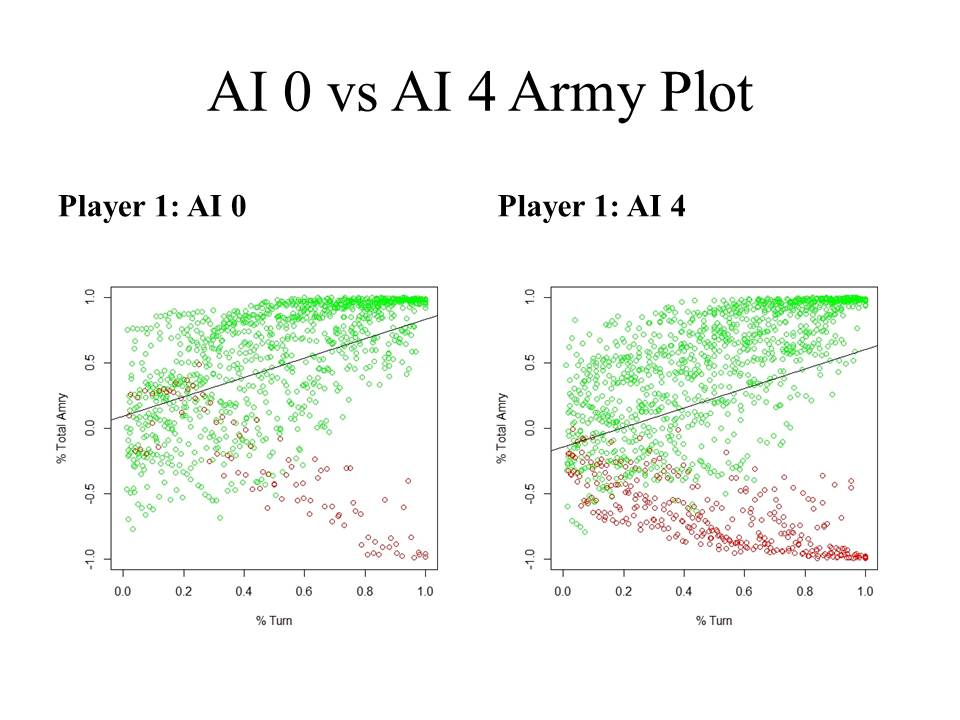
\includegraphics[scale=0.6]{images/Figure_1.jpg}\\
{\footnotesize Figure 1.}
\end{center}

Here the green and red dots represent AI0’s and AI4’s percent total armies respectively over time. Again, the dots only represent games in which a definitive winner was found. Here we see that AI0 has a clear advantage but when the player order is changed, AI4 wins more games. Notice, however, while the trend line shifts down, that the slope stays constant. This implies that while the game is certainly affected by player order, on average, the game develops the same regardless of player order. 

For the same AI match, the fun function provides two survival charts. Now consider figure 2. 


\begin{center}
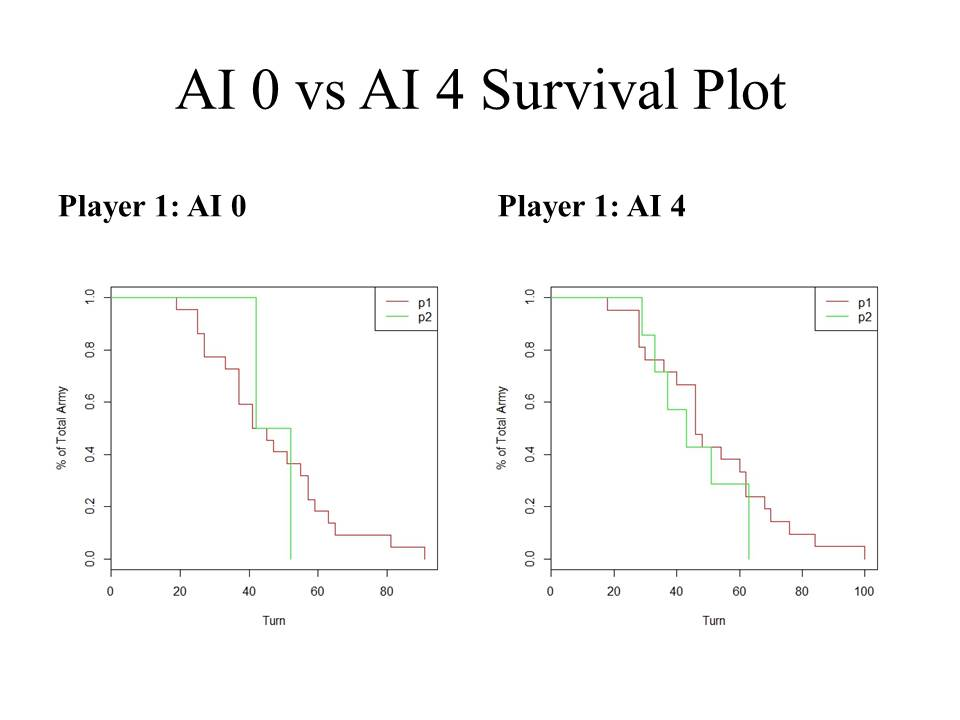
\includegraphics[scale=0.6]{images/Figure_2.jpg}\\
{\footnotesize Figure 2.}
\end{center}

In the first plot we see that player two holds several armies until near round 50. Suddenly over the next two rounds however, we see an incredible drop off. AI0 has mostly defensive characteristics. From this it appears that AI0 condenses its portion of the graph and builds armies. Somewhere near halfway through the game, it branches out and gains several territories in a very small period of time. When the order of the game is reversed we see a much more even trend. Both AI’s seem to lose armies at a consistent rate. This effect could be accredited to player order effect or the characteristics of the players in regards to their section of the sub graph. 


While these trends, in general, hold true, one AI in particular defied the general trends. We will call this AI, AI3. AI3, in general, tended to produce more wins when playing in the second player position. This trend was tested more rigorously against 15 new AI’s. From this data, the fun function produced the win records for both AI3 and the other AI’s for both player order. The difference between wins was then calculated. That is $\Delta \emph{win} = \emph{AI3\_wins} - \emph{AIOpponent\_wins}$. This figure was calculated for both player orders. This data is represented in figure 3.



\begin{center}
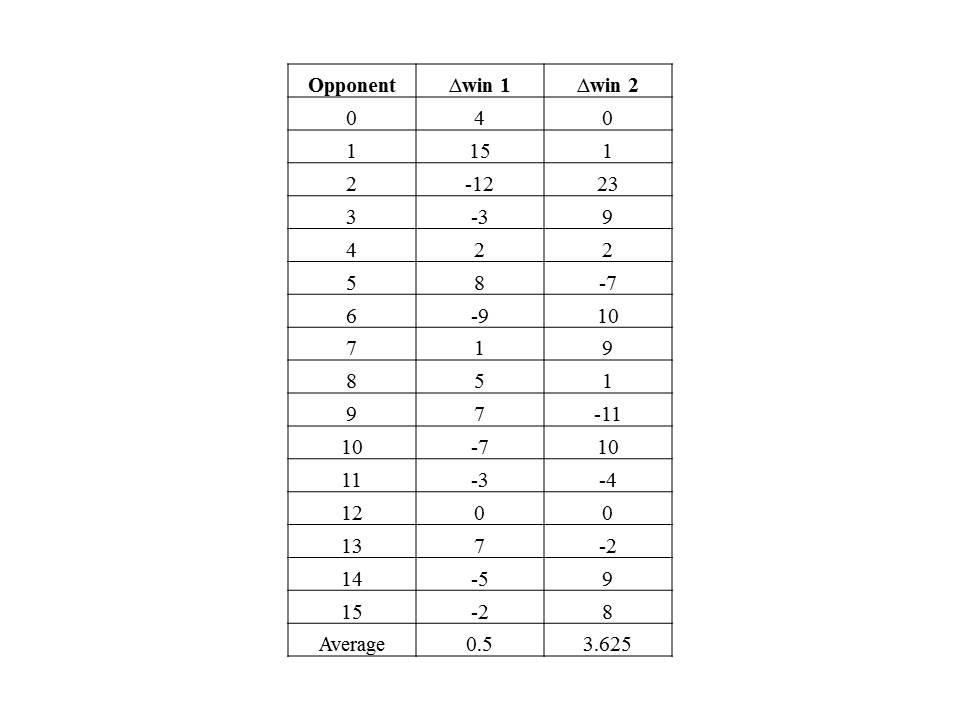
\includegraphics[scale=0.6]{images/Figure_3.jpg}\\
{\footnotesize Figure 3.}
\end{center}


As in figure 3, on average AI3 wins 3.625 games while playing second in comparison to playing first where the AI won only 0.5 games on average. This in turn would seem to offer a solution to the player order effect, mentioned above. By simply playing the AI3 characteristics (“Survival”, “Defensive”, “Cautious”, “Carry”), on average the advantage would go to the second player, thus making player order obsolete. 


Another nuanced observation shows that this conclusion may not be entirely true. Under further observation, another AI which we will call AI4 (“Survival”, “Aggressive”, “Tactical”, “Rusher”) seemed to be superior to AI3 in both player orders. A more rigorous study of these two AI’s revealed that the assumption was correct. The fun function showed that on average, AI4 wins more often than AI3. Consider figure 4 and figure 5. 



\begin{center}
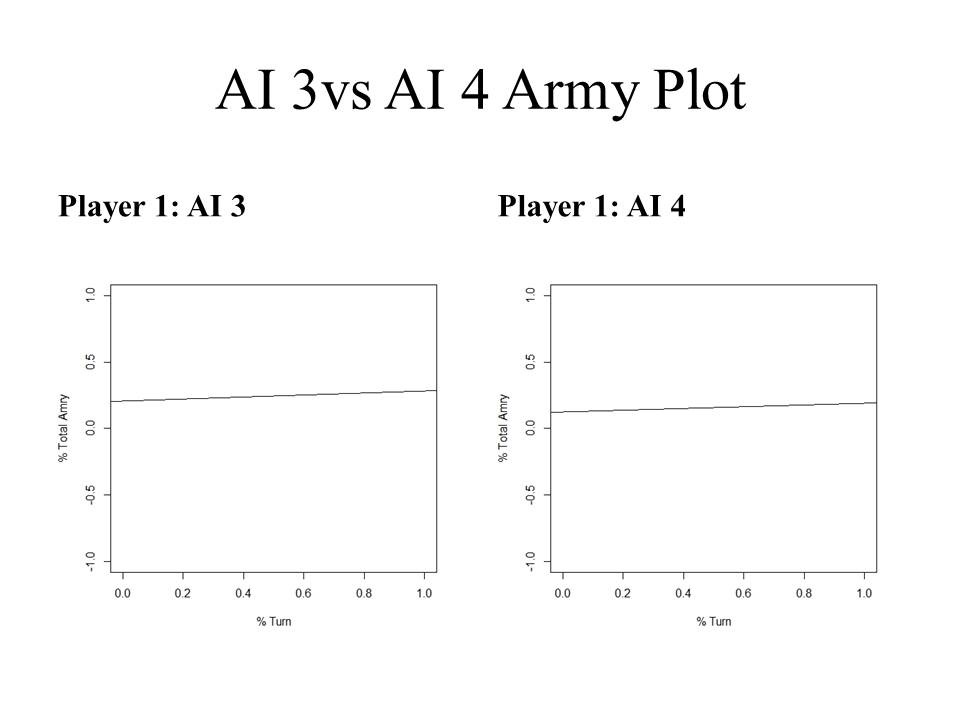
\includegraphics[scale=0.6]{images/Figure_4.jpg}\\
{\footnotesize Figure 4.}\\
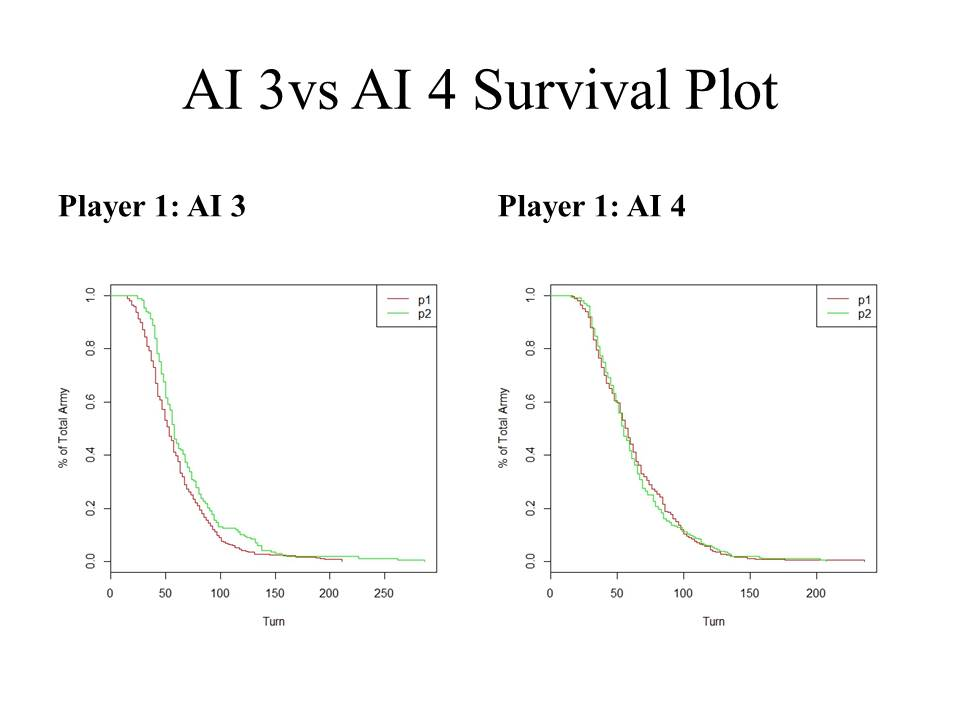
\includegraphics[scale=0.6]{images/Figure_5.jpg}\\
{\footnotesize Figure 5.}
\end{center}

Notice that these two figures show very low correlation when player order changes. When AI3 goes first, it grosses more wins than AI4. When AI3 goes second, however, AI4 wins the majority of the games. While by a narrow margin, when AI4 goes first, AI4 wins 56 more games than AI3 in a 500 game trial. Thus if AI3 plays second they will on average lose to AI4. 


\subsection{AI behaviors and Surprises}
In this project several AI’s were posed against each other in a game of Risk. Initially, it was predicted that a large player order effect would affect the game. This hypothesis held true for the majority of AI’s that were tested in this experiment. AI3 however, proved that by using the correct strategy, a player would actually hold an advantage by going second in the game. From this however, AI4 proved that their still exist AI’s that can beat AI3 while being the first player to move. 

From this project, we advise future Risk players to abstain from declaring their player strategy until the player order is determined. From this, we advise that second players play a cautious, defensive game, while first players play with aggressive tendencies. A consistent analysis of strategy will reveal the best strategy for either player to take throughout the duration of the game. 



\section{Conclusion}
We have reformalized the board game \emph{Risk} as a graph optimization, and implemented an AI to solve the problem, i.e. to play the game. Several decision algorithms were devised based on graph properties, and they in turn form the personalities of the AI. Our study of 4 binary traits, or a total of 16 personality variations of the AI, is merely the beginning. We have discovered some interesting AI behaviours and performance at a level beyond any human players. One can potentially investigate even more variations of the traits.

For future studies, an analysis of subgraphs would provide deep insight into the value of individual territories. The AI’s are built in such a way that the priority function is based off of current demographic of troops and shape of their graph. Evaluating the graph as a whole would provide insight to the value of different subgraphs that would proactively affect the priority function. This conditional thinking is much more like the ideas of a human player and thus could inform future strategies. 

Furthermore, game shifts could be analyzed using the fun function and the aforementioned subgraph analysis. This would allow for defensive players an understanding of which territories that are worth defending and worth conceding. This shift parameter would allow for insight to game length, army distribution, and other key factors.  





\section{Citations}

Hasbro, \emph{Risk, The World Conquest Game \circledR, Rules ©1959, 1963, 1975, 1980, 1990, 1993}, Parker Brothers, Division of Tonka Corporation, Beverly, MA 01915, U.S.A.




\end{document} 

